\documentclass[]{article}

\usepackage{graphicx}

%opening
\title{}
\author{}

\begin{document}

\maketitle

\begin{abstract}

\end{abstract}

\section{Base Sequool}
The idea is to compute an index $ind(n)$ for a node $n$ that measures the minimum amount of change  in the value of all the nodes such that this node $n$ becomes the best.

This can be computed recursively as :
$$ind(n) = max( ind(parent(n),.5*abs(value(n)-value(parent(n)))) $$

\section{another}
The idea is to compute an index $ind(n)$ for a node $n$ that measures the minimum amount of change  in the value of  the node $n$ alone such that this node $n$ becomes the best.
In some case is undefined as with any amount of change the node remains suboptimal. For instance in the example below
the node with value cannot be changed alone to be best

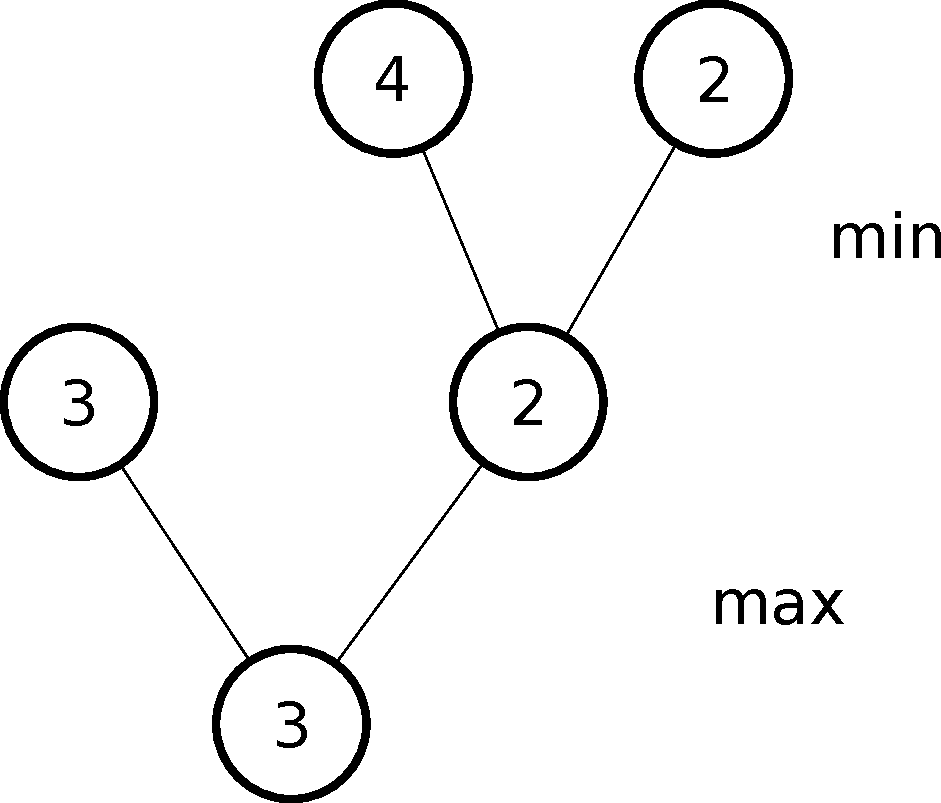
\includegraphics[width=4cm]{treeanother}


This can be computed recursively as :
$$ind(n) =  $$

\end{document}
